\documentclass[paper=a4,fontsize=11pt]{temp} % KOMA-article class                            
\begin{document}

\begin{minipage}{.2\linewidth}
   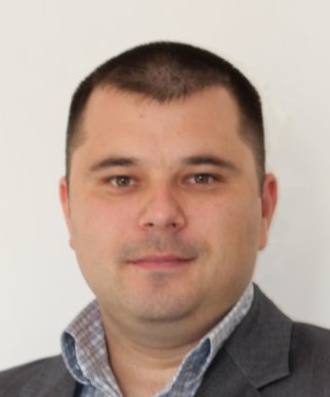
\includegraphics[width=1\textwidth]{IMG/photo}
\end{minipage}      
\begin{minipage}{0.7\linewidth}
   \MyName{Yaroslav Shumlianskyi}
   \sepspace
   \noindent
   
   \hfill shumliankyi@ukr.net

   \hfill i.am.LLluma@gmail.com  

   \hfill www.linkedin.com/in/yaroslav-shumlianskyi
   
 
\end{minipage}

\NewPart{Summary}{}

A qualified engineer with 11+ years of commercial experience in software development accompanied by technical
leadership.
Primary competence comprises Python, BigData, and related technology stack applied to automotive and IT domains.
Solid expertise in communicating with project stakeholders, planning and estimating development efforts, coordinating
cross-team activities, as well as monitoring quality control processes.
Eager to advance my expertise in Go, Spark/Scala, and machine learning best practices.


\NewPart{Work experience}{}

\noindent


\workEntry{Fintech, Data lake}{Jun 2017 - Present}{Lead Python Developer} 
{The customer is a leading innovator for digital financial services and helps to create better banking for a digital world.
The company has designed an innovative digital platform, that uses open APIs and quickly became a breakthrough for
next-generation banking. They provide existing financial, retail, and telecom institutions — as well as startup banks —
the chance to bring digital technology to the heart of their businesses.}
{
\begin{itemize}
    \setlength\itemsep{0em}
    \item Projecting and developing a distributed Data lake system based on Spark 
    \item Deploying Data lake system with using Infrastructure as code approach (Ansible/Docker Swarm)
    \item Organizing ETL pipelines with using Apache AirFlow platform
\end{itemize}
}
{Python, Spark, PySpark, SparkSQL, AirFlow, Ansible, Docker, SageMaker}
{IMG/intellias}
{Intellias}

\sepspace

\workEntry{Map data testing framework}{Dec 2015 - Jun 2017}{Lead Python Developer} 
{The customer, a global provider of map solutions, navigation systems, and location-based services, requested to
optimize the performance of their framework that would enable fast, reliable, and qualitative testing of map data. The
developed solution allowed reducing expensive recalls, delivering better quality maps and made the process of map
releasing much faster. The system used reference tests based on comparative analysis of data retrieved from compilation
data sources against compiled data as well as non-reference tests based on the analysis of compiled data only.
Optimization of the framework performance included the development of new functionality and migration to Cassandra and
Elastic MapReduce.}
{
\begin{itemize}
    \setlength\itemsep{0em}
    \item Communicated with the stakeholders to define project requirements
    \item Coordinated cross-team communication and collaboration
    \item Migrated the framework from CouchDB to Cassandra
    \item Performed the product migration from Hadoop to Elastic MapReduce
    \item Created a Python wrapper for S3 files
    \item Performed code reviews
\end{itemize}
}
{Python, Cython, C++, Python wrappers, Hadoop, Spark, Jenkins, Ansible, Boto 3, Cassandra, CouchDB}
{IMG/intellias}
{Intellias}

\sepspace
\clearpage

\workEntry{ERP system}{Dec 2011 - Jun 2015}{Team Leader, Solution Architect} 
{The product was delivered for a UK-based provider of fully customizable business management solutions intended to meet
requirements of small- and medium-sized companies. It was a multimodular ERP system that included accounting,
purchases, production, sales, CRM, warehouse, project, and service management. The developed solution reduced
duplication of processes, improved inter-departmental communication, increased process flexibility, as well as provided
robust business analytics.
The scope of the project encompassed the extension of the existing functionality and migration to new technologies, such as
Ansible and Robot Framework.}
{
\begin{itemize}
    \setlength\itemsep{0em}
    \item Optimized performance of OpenERP ORM, making it more lightweight and reducing the number of writes/reads to a database while
performing business operations
    \item Fine-tuned the PostgreSQL server performance
    \item Developed new and modified the existing functionality for processing a huge amount of input data
    \item Integrated OpenERP with the Magento eCommerce platform
    \item Managed the process of product support, monitoring, and solving critical issues
    \item Coordinated the software releases
\end{itemize}
}
{Python, OpenERP, Werkzeug, Flask, Barman, PostgreSQL}
{IMG/enapps}
{Enapps Ltd}

\sepspace

\workEntry{Geoinformation management system}{Aug 2004 - Dec 2011}{\ldots} 
{The project was intended for a Ukraine’s governmental institution dealing with visualization, management, and analysis
of geographic data. The product under development was a geoinformation system (GIS) used for acquisition, storage,
analysis and graphic visualization of geospatial data. The solution was graphically oriented and enabled designing and
presenting various maps, photographs, illustrations, histograms, and results of statistic surveys.}
{
\begin{itemize}
    \setlength\itemsep{0em}
    \item Conducted a profound study and analysis of imagery and geospatial data 
    \item Described, evaluated and visualized physical features (places) and geographically localized processes on the
        Earth's sphere
    \item Performed archiving and cataloging of raw geospatial data and results of its processing
    \item Prepared technical documentation according to the results of geospatial data analysis
\end{itemize}
}
{Python, ArcGIS, IDL, ENVI}
{IMG/globe}
{Ukraine’s governmental institution}

\sepspace


\NewPart{Education}{}
\noindent


\EducationEntry{Master of Science - MS}
{1999 - 2004}
{Zhytomyr Military Institute named after S.Korolyov}
{Radio Electronics, Processing of Remote Sensing Data}
{IMG/zvir}

\sepspace

\NewPart{Skills}{}
\hspace{3mm}
\begin{minipage}[t]{0.5\textwidth} 

\begin{tabular}[t]{ l l }
\flag{IMG/gb}  & Upper Intermediate \\
\end{tabular}

\sepspace

\end{minipage}
%
\begin{minipage}[t]{0.5\textwidth} 


\begin{tabular}[t]{l l}
\software{IMG/python}           & Python\\
\software{IMG/javascript}      & JavaScript\\
\software{IMG/tdd}           & TDD\\
\software{IMG/bigdata}         & Big Data\\
\software{IMG/devops}          & DevOps\\
\end{tabular}



\end{minipage}


%%% References
%%% ------------------------------------------------------------

\end{document}
